\documentclass[]{article}
\usepackage[margin=0.5in]{geometry}
\usepackage{amsthm}
\usepackage{mathtools}
\usepackage{amsfonts}
\usepackage{multicol}
\usepackage{tikz}
\usepackage{eurosym}
\usepackage{algorithm}
\usepackage{algorithmicx}
\usepackage{algpseudocode}
\DeclareRobustCommand{\officialeuro}{%
	\ifmmode\expandafter\text\fi
	{\fontencoding{U}\fontfamily{eurosym}\selectfont e}}
\usepackage{caption}
\usepackage{subcaption}
\usetikzlibrary{matrix}
\usepackage{ stmaryrd }
\newtheorem{definition}{Definition}[section]
\newtheorem{theorem}{Theorem}[section]
\newtheorem{lemma}[theorem]{Lemma}
\newtheorem{conjecture}[theorem]{Conjecture}
\usepackage[toc,page]{appendix}
\usepackage{forest}



\begin{document}
\begin{algorithm}
	\caption{$\textsc{RecursivePG}(\textit{PG } G = (V,V_0,V_1, E, \Omega))$}
	\label{alg_zlnk_org}
	\begin{algorithmic}[1]
		\State $m \gets \min\{ \Omega(v)\ |\ v \in V\}$
		\State $h \gets\max\{ \Omega(v)\ |\ v \in V\}$
		\If{$h = m$ or $V = \emptyset$}
		\If{$h$ is even or $V = \emptyset$}
		\State \Return $(V,\emptyset)$
		\Else
		\State \Return $(\emptyset, V)$
		\EndIf
		\EndIf
		\State $\alpha \gets 0$ if $h$ is even and $1$ otherwise
		\State $U \gets \{v \in V\ |\ \Omega(v) = h\}$
		\State $A \gets \alpha\textit{-Attr}(G, U)$
		\State $(W_0', W_1') \gets \textsc{RecursivePG}(G \backslash A)$
		\If{$W_{\overline{\alpha}}' =\emptyset$}
		\State $W_\alpha \gets A \cup W_\alpha'$
		\State $W_{\overline{\alpha}} \gets \emptyset$
		\Else
		\State $B \gets \overline{\alpha}\textit{-Attr}(G,W_{\overline{\alpha}}')$
		\State $(W_0'', W_1'') \gets \textsc{RecursivePG}(G \backslash B)$
		\State $W_\alpha \gets W_\alpha''$
		\State $W_{\overline{\alpha}} \gets W_{\overline{\alpha}}'' \cup B$
		\EndIf
		\State \Return $(W_0, W_1)$
	\end{algorithmic}
\end{algorithm}
\begin{conjecture}
	For any $\textsc{RecursivePG}(G')$ that is invoked during $\textsc{RecursivePG}(G)$ it holds that any vertex $v \in W'_{\overline{\alpha}}$ is won by player $\overline{\alpha}$ in game $G$.
\end{conjecture}
Counter example $G$:\\
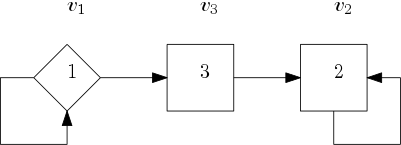
\includegraphics[scale=0.5]{counterexampleBconjecture}\\
All vertices are won by player $0$.\\
$\textsc{RecursivePG}(G)$:\\
$h=3$,$\alpha=1$\\
$A =\{v_3\}$\\
\begin{tabular}{|p{20cm}}
$\textsc{RecursivePG}(G\backslash A)$:\\
$\hat{h}=2,\hat{\alpha}=0$\\
$\hat{A}=\{v_2\}$\\
\begin{tabular}{|p{20cm}}
$\textsc{RecursivePG}(G\backslash A\backslash \hat{A})$\\
\end{tabular}
$\hat{W}'_0 = \emptyset$\\
$\hat{W}'_1 = \{v_1\} = \hat{W}'_{\overline{\hat{\alpha}}}$\\
\textbf{Vertex $v_1$ is in $\hat{W}'_{\overline{\hat{\alpha}}}$ however in $G$ the vertex is won by player} $\hat{\alpha}$.\\
$\hat{B} = \{v_1\}$\\
\begin{tabular}{|p{20cm}}
$\textsc{RecursivePG}(G\backslash A\backslash \hat{B})$\\
\end{tabular}
$\hat{W}''_0 = \{v_2\}, \hat{W}''_1 = \emptyset$\\
\end{tabular}
$W'_0 = W'_{\overline{\alpha}} = \{v_2\}$\\
$W'_1 = W'_\alpha = \{v_1\}$\\
$B = V$\\
$W_0 = V$
\end{document}
